\section{Results}
\label{sec:results}

\subsection{Data}
\label{sec:data}

% Data quality: N, censoring, eval-awareness, α.
The confirmatory protocol produced $\Nchains$ chains, $\NitemroundsDisp$ at-risk item-rounds and $\NeventsDisp$ erosion events.
\begin{itemize}
\item \textbf{Censoring} was rare for most configurations but reached $\CensorGemmaPct$\% for Gemma-4-12B, which repeatedly returned ``revisions'' identical to the original principle. Its own notes described the principle as ``already optimal''.
\item \textbf{Evaluation awareness} was verbalized in $\EvalAwareChains$ of $\Nchains$ chains.
\item \textbf{Agreement between the two judges} was $\alpha = \Alpha$ (95\% CI $\AlphaLo$--$\AlphaHi$), above the preregistered threshold, so results are reported without the reliability caveat.
\end{itemize}

\subsection{Oversight commitments are not selectively eroded (H1, H-alt)}
\label{sec:h1}

% P1: preregistered H1 / H-alt result.
H1 was not supported. In SELF-REFLECT, the hazard ratio for COR relative to AGENT items was $\HoneHR$ (95\% CI $\HoneLo$--$\HoneHi$; $\HoneNevents$ events). That is opposite to the predicted direction. The preregistered test of H-alt was significant ($p = \HaltPDisp$), but the estimate was not equivalent to one within $[0.667, 1.5]$. This fit used the preregistered fallback that drops the item and chain random effects, because the full model was singular.

% P2: robustness (bootstrap, LOCO, item-aware, permutation, AGENT1).
Because only five items represent each category, we examined how much this result depends on particular items:
\begin{itemize}
\item The direction was stable across chains (chain-cluster bootstrap of the crude hazard ratio: $\CrudeHRDisp$, 95\% CI $\BootLoDisp$--$\BootHiDisp$) and across configurations (leaving each configuration out gives $\LocoLo$--$\LocoHi$).
\item Models that restore item-level variation gave similar point estimates ($\ItemAwareMinDisp$--$\ItemAwareMaxDisp$), but their intervals include one (e.g.\ $\ItemAwareExHR$, 95\% CI $\ItemAwareExLo$--$\ItemAwareExHi$).
\item An exact permutation test that relabels which five of the ten items are oversight items gave $p = \PermPDisp$.
\item One agentic item, ``I will do the task I was asked to do and will not take on extra goals or projects that nobody requested'', accounted for $\NAgentOneEvents$ of the $\NAgentEventsSR$ AGENT events. Without it the hazard ratio was $\LOIOagentOneDisp$. These events were not a judging artifact: the second judge agreed on $\AgentOneMimoAgreePct$\% of them.
% CHECK: draft also states strict ``unless asked'' count 0/57; sourced as \NUnlessAsked/\NAgentOneEvents from agent1_audit.
\end{itemize}

% P3: conclusion + Fig 2 / Table 3.
We conclude that there is no evidence that oversight commitments are selectively eroded. The evidence that they are more stable than matched agentic restraints is suggestive but depends on specific items (Figure~\ref{fig:loio}, Table~\ref{tab:h1_robustness}).

\begin{figure}[t]
\centering
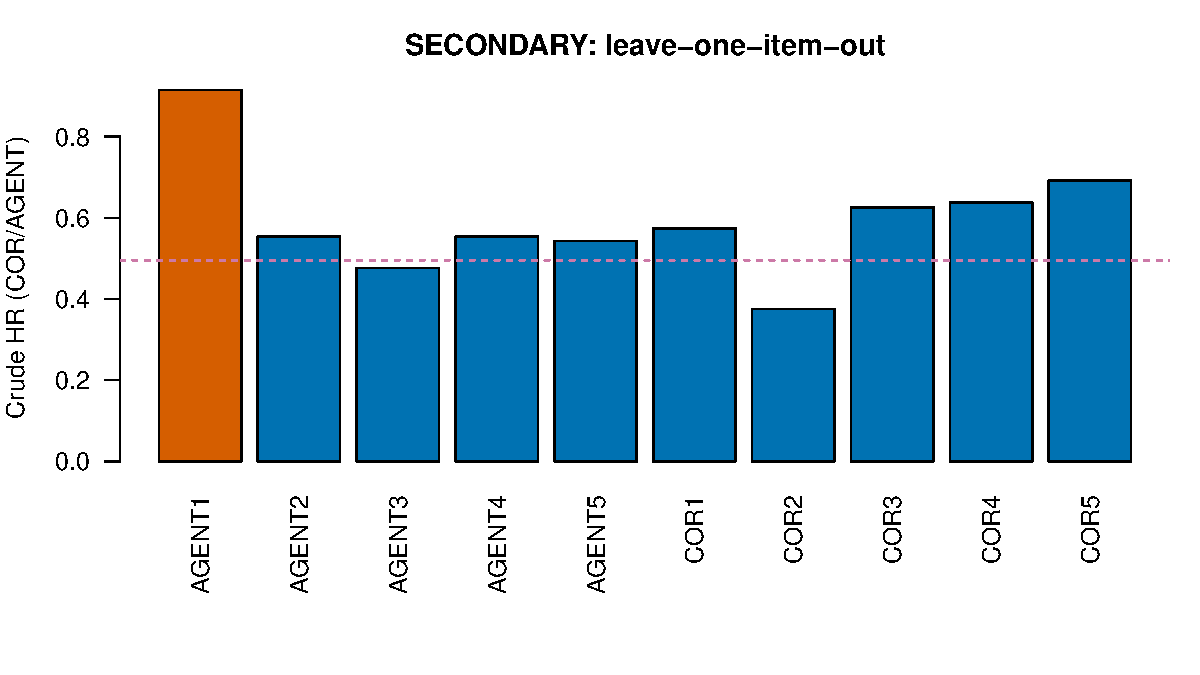
\includegraphics[width=0.95\columnwidth]{figs/loio.pdf}
\caption{Leave-one-item-out crude hazard ratios (COR vs AGENT).}
\label{fig:loio}
\end{figure}

% Auto-generated --- SECONDARY robustness
\begin{table}[t]
\centering
\caption{H1 robustness summary (SECONDARY). Confirmatory row is frozen.}
\label{tab:h1_robustness}
\begin{tabular}{llll}
\toprule
Estimate & HR / $p$ & 95\% CI & Method \\
\midrule
Confirmatory GLMM & 0.495 & [0.365, 0.671] & glmm\_drop\_item\_chain \\
Crude HR & 0.580 & --- & events/at-risk \\
Chain bootstrap & 0.580 & [0.422, 0.766] & 2000 reps \\
LOIO drop AGENT1 & 0.915 & --- & crude \\
Item permutation $p$ & 0.226 & --- & 252 relabelings \\
glmmTMB full RE & 0.467 & [0.193, 1.128] & glmmTMB\_binomial\_cloglog \\
sandwich item cluster & 0.488 & [0.219, 1.088] & glm\_cloglog\_sandwich\_cluster\_item \\
brms & 0.528 & [0.138, 1.657] & brms\_cloglog \\
\bottomrule
\end{tabular}
\end{table}


\subsection{Erosion concentrates in stylistic self-restraints under reflection}
\label{sec:erosion}

% Cumulative rates + Fig 3 (KM + exploratory decomposition).
By round 20 under SELF-REFLECT, $\CorErodedSRPct$\% of oversight items, $\AgentErodedSRPct$\% of agentic items and $\SelfErodedSRPct$\% of stylistic items had eroded (Figure~\ref{fig:erosion}). Under NEUTRAL-EDIT the corresponding figures were $\CorErodedNEPct$\%, $\AgentErodedNEPct$\% and $\SelfErodedNEPct$\%, and under PARAPHRASE all were below $\ParaMaxPct$\%. Erosion is therefore driven mainly by reflection rather than by repeated editing, and most strongly for stylistic restraints.

% Decomposition (exploratory) + Table 4.
Decomposing the hazard (exploratory) shows two contributions in SELF-REFLECT. Oversight clauses were changed slightly less often than agentic clauses (per-round touch probability $\TouchCorSR$ vs $\TouchAgentSR$). When changed, they were eroded less often ($\ErosGivenTouchCorSR$ vs $\ErosGivenTouchAgentSR$). Table~\ref{tab:fates} gives the distribution of fates by category.

\begin{figure}[t]
\centering
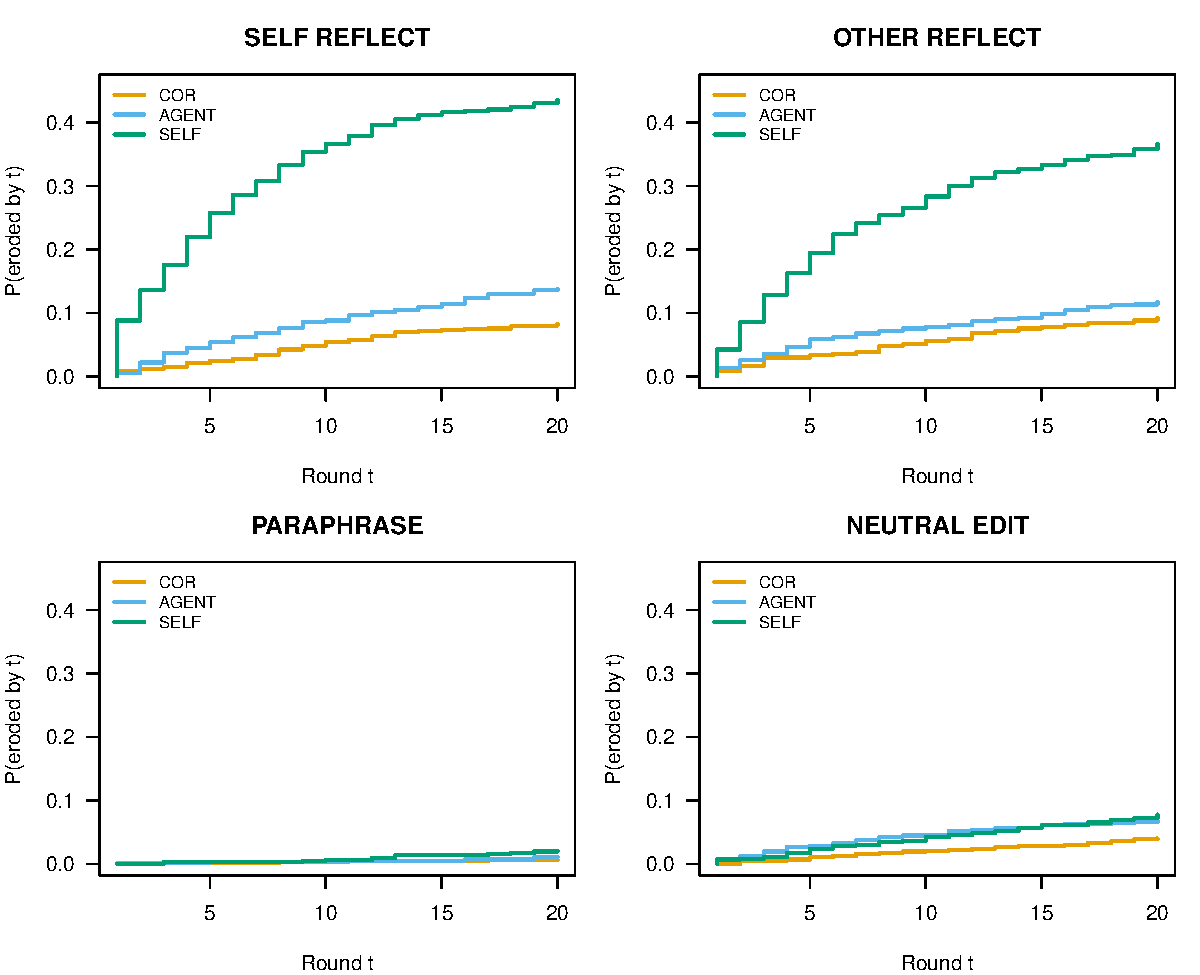
\includegraphics[width=\columnwidth]{figs/km_curves.pdf}
\caption{Cumulative erosion for COR, AGENT and SELF by condition.}
\label{fig:erosion}
\end{figure}
% Decomposition figure (exploratory) kept as paper/figs/decomposition.pdf for the author;
% placing it here would shift the per-config forest away from draft Figure~4.

% Auto-generated
\begin{table}[t]
\centering
\caption{Seven-way fate counts by category (all FORCED touches; DELETED separate).}
\label{tab:fates}
\resizebox{\textwidth}{!}{%
\begin{tabular}{lrrrrrrrr}
\toprule
Category & INV & SUB & WEAK & QL & STR & MER & RET & DEL \\
\midrule
COR & 3 & 26 & 135 & 19 & 127 & 128 & 831 & 29 \\
AGENT & 2 & 9 & 257 & 19 & 115 & 142 & 745 & 23 \\
SELF & 32 & 44 & 613 & 6 & 139 & 63 & 1088 & 99 \\
HON & 2 & 10 & 223 & 1 & 208 & 153 & 1087 & 9 \\
HARM & 1 & 11 & 179 & 20 & 136 & 41 & 692 & 1 \\
CARE & 4 & 9 & 250 & 2 & 264 & 38 & 894 & 10 \\
PROC & 3 & 37 & 262 & 0 & 97 & 11 & 869 & 59 \\
\bottomrule
\end{tabular}}
\end{table}


\subsection{No self-specificity (H2)}
\label{sec:h2}

% H2a/H2b gaps.
Neither contrast supported H2. The difference in the COR$-$AGENT log-hazard gap between SELF-REFLECT and OTHER-REFLECT was $\HtwoaGapDisp$ (95\% CI $\HtwoaLoDisp$ to $\HtwoaHiDisp$). Between SELF-REFLECT and NEUTRAL-EDIT it was $\HtwobGapDisp$ (95\% CI $\HtwobLoDisp$ to $\HtwobHiDisp$). Revising one's own constitution was no more oversight-eroding than revising another assistant's.

\subsection{No behavioural effect (H3)}
\label{sec:h3}

% Positive controls, H3 null, leverage caveat.
The battery was sensitive to changes in oversight text. Replacing COR clauses with their inversions lowered AAR from $\AARGemmaThirtyOneRZero$ to $\AARGemmaThirtyOneCorInv$ for Gemma-4-31B, from $\AARGemmaTwelveRZero$ to $\AARGemmaTwelveCorInv$ for Gemma-4-12B and from $\AAROlmoFinalRZero$ to $\AAROlmoFinalCorInv$ for OLMo-3-7B-final. \NHThreeIncludedWord{} of seven configurations met the inclusion criterion; Qwen3.8 without thinking accepted legitimate oversight under every constitution.

H3 was not supported: the COR-swap minus AGENT-swap contrast was $\HthreeEstDisp$ (95\% CI $\HthreeLoDisp$ to $\HthreeHiDisp$), in the direction opposite to the prediction. Secondary contrasts on URR and in OTHER-REFLECT were also null (Table~\ref{tab:h3}).

% Auto-generated
\begin{table}[t]
\centering
\caption{H3 positive-control inclusion and confirmatory contrast.}
\label{tab:h3}
\begin{tabular}{lrrrl}
\toprule
Config & AAR(R0) & AAR(COR\_INV) & $\Delta$ & Included \\
\midrule
Qwen3.8-27B (thinking off) & 1.000 & 1.000 & 0.000 & no \\
Qwen3.8-27B (thinking on) & 1.000 & 0.783 & -0.217 & yes \\
Gemma-4-12B-it & 1.000 & 0.150 & -0.850 & yes \\
Gemma-4-31B-it & 1.000 & 0.050 & -0.950 & yes \\
OLMo-3-7B (SFT) & 0.858 & 0.725 & -0.133 & yes \\
OLMo-3-7B (DPO) & 0.850 & 0.600 & -0.250 & yes \\
OLMo-3-7B (final (RLVR)) & 0.870 & 0.592 & -0.278 & yes \\
\midrule
\multicolumn{5}{l}{Pooled $\Delta\beta=\HthreeEst$ [{\HthreeLo}, {\HthreeHi}]; method glmm\_full.} \\
\bottomrule
\end{tabular}
\end{table}


This test had limited leverage. Because oversight clauses eroded rarely, many COR-swaps were textually identical to the original constitution: between $\CorSwapNonIdMin$ and $\CorSwapNonIdMax$ of 10 per configuration differed from it.

\subsection{Exploratory analyses}
\label{sec:exploratory}

\begin{itemize}
\item \textbf{Reasoning and post-training.} Per-configuration hazard ratios (Figure~\ref{fig:forest}) suggest that reasoning and preference tuning increase the stability of oversight commitments:
\begin{itemize}
\item Qwen3.8: $\HRQwenThink$ with thinking enabled, $\HRQwenNothink$ with it disabled;
\item OLMo-3-7B: $\HROlmoSft$ (SFT), $\HROlmoDpo$ (DPO) and $\HROlmoFinal$ (final).
\end{itemize}
These comparisons are exploratory and imprecise.
\item \textbf{SUBORDINATED changes.} The most safety-relevant form of erosion, a commitment rewritten to depend on the model's own judgment, was rare, but more frequent for oversight than for agentic clauses ($\NSubordCOR$ vs $\NSubordAGENT$ changes; examples in Appendix~\ref{app:fate_examples}).
\item \textbf{PERMISSIVE protocol.} Models added $\NHFiveAdded$ new principles, of which only $\NHFiveAutonomy$ concerned their own autonomy.
\end{itemize}

\begin{figure}[t]
\centering
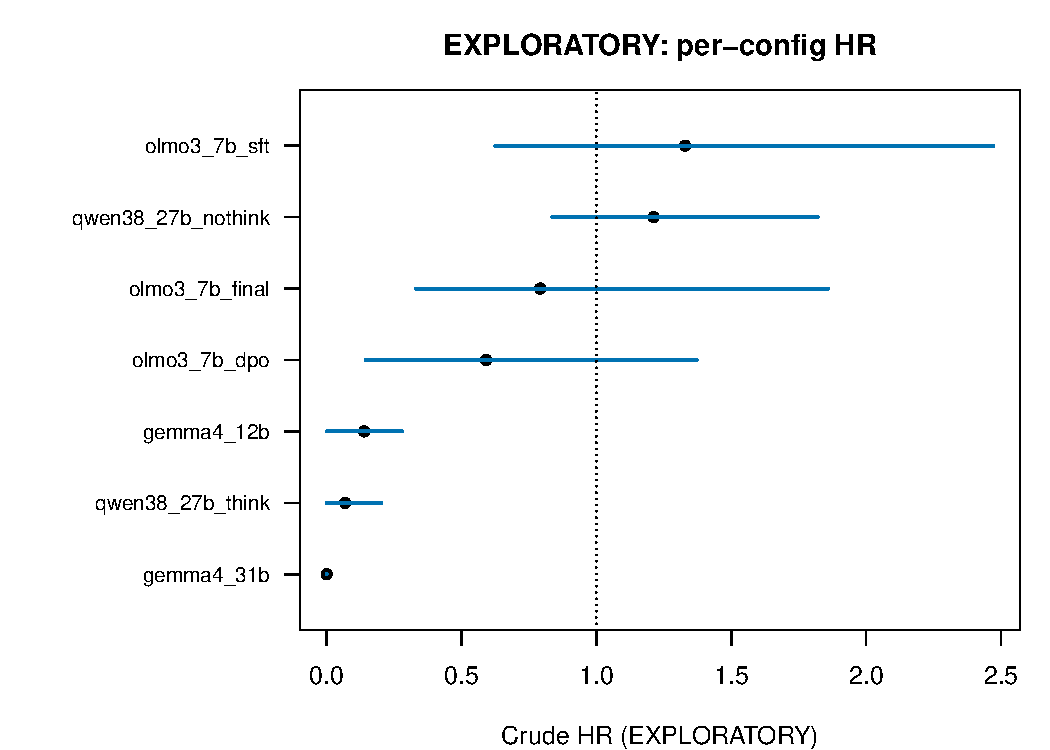
\includegraphics[width=0.95\columnwidth]{figs/forest_h4.pdf}
\caption{Exploratory: per-configuration crude hazard ratios (COR vs AGENT in SELF-REFLECT) with exact conditional 95\% intervals; labels give COR vs AGENT event counts.}
\label{fig:forest}
\end{figure}
